\documentclass{article}
%%%%%%%%%%%%%
% Loads packages
%%%%%%%%%%%%%
\usepackage[table]{xcolor}
\usepackage[utf8]{inputenc}
\usepackage[colorlinks=true,linkcolor=blue]{hyperref}
\usepackage{geometry} %package needed to set margins
\usepackage{fancyhdr}
\usepackage{graphicx}
\usepackage{amsmath}
\usepackage{amsthm}
\usepackage{mdframed}
\usepackage{tikz}
\usetikzlibrary{patterns}
\usepackage{amsfonts}

\pagestyle{fancy}
\fancyhf{}
\chead{\textbf{Homework 1}}
\lhead{Math 213-A1, Spring 2026}
\rhead{Due Friday, 1/30 at 9:00am}

%%%%%%%%%%%%%
% Sets margins
%%%%%%%%%%%%%
\newgeometry{left=1.5in,right=1in,top=1in,bottom=1in}
\setlength\headsep{3pt}

%%%%%%%%%%%%%
% Creates problem and solution environments
%%%%%%%%%%%%%

% Solution Environment
\newenvironment{solution}{\begin{proof}[Solution]}{\end{proof}}

% Problem Environment
\newenvironment{problem}[1]
    {\begin{mdframed}[default]
    \textbf{Problem #1:}
    }
    {\end{mdframed}
    }
    
%%%%%%%%%%%
% Custom Commands
%%%%%%%%%%%
\newcommand{\gOne}{\cellcolor{green!50!white} 1}
\newcommand{\rZero}{\cellcolor{red!50!white} 0}

\begin{document}

\begin{problem}{\S 1.1: 8(a,d,f,h)}
Let $p$ and $q$ be the propositions
\begin{align*}
&\text{$p$: I bought a lottery ticket this week.}\\
&\text{$q$: I won the million dollar jackpot.}
\end{align*}
Express each of these propositions as an English sentence.
\begin{enumerate}
    \item[(a)] $\neg p$
    \item[(d)] $p\land q$
    \item[(f)] $(\neg p) \implies (\neg q)$
    \item[(h)] $(\neg p) \lor (p\land q)$
\end{enumerate}
\end{problem}

\begin{solution}
Below are the propositions in plain English
\begin{enumerate}
    \item[(a)] I didn't buy a lottery ticket this week.
    \item[(d)] I bought a lottery ticket this week and I won the million dollar jackpot.
    \item[(f)] If I didn't buy a lottery ticket this week, then I didn't win the million dollar jackpot.
    \item[(h)] I either didn't buy a lottery ticket this week or I bought one and won the million dollar jackpot.
\end{enumerate}
\end{solution}

\begin{problem}{\S 1.2: 6}
Use a truth table to verify the first De Morgan law $\neg (p\land q) \equiv \neg p \lor \neg q$.
\end{problem}

\begin{solution}
\begin{tabular}{ccccccc}
$p$ & $q$ & $p \land q$ & $\neg ( p \land q)$ & $\neg p$ & $\neg q$ & $\neg p \lor \neg q$ \\
\hline\\
1 & 1 & 1 & 0 & 0 & 0 & 0\\
1 & 0 & 0 & 1 & 0 & 1 & 1\\
0 & 1 & 0 & 1 & 1 & 0 & 1\\
0 & 0 & 0 & 1 & 1 & 1 & 1
\end{tabular}

\end{solution}

\begin{problem}{\S 1.4: 14(a,d)}
Express each of these quantifications in English, if the domain consists of all real numbers. Then, determine the truth value of the statement
\begin{enumerate}
    \item[(a)] $\exists x(x^3=-1)$
    \item[(d)] $\forall x(2x>x)$
\end{enumerate}
\end{problem}
\begin{solution}
Here are the quantifications in English
\begin{enumerate}
    \item[(a)] There exits an $x$; and the statement is True
    \item[(d)] For all $x$; and the statement is False
\end{enumerate}
\end{solution}

\begin{problem}{\S 2.1: 10(a,c,e,g)}
Determine whether the following statements are true or false.
\begin{enumerate}
    \item[(a)] $\emptyset \in \{ \emptyset \}$
    \item[(c)] $\{ \emptyset \} \in \{ \emptyset \}$
    \item[(e)] $\{ \emptyset \} \subset \{ \emptyset, \{ \emptyset \} \}$
    \item[(g)] $\{ \{ \emptyset \} \} \subset \{ \{ \emptyset \}, \{ \emptyset \} \}$
\end{enumerate}
\end{problem}

\begin{solution}
 Is an element of and is a subset of.
\begin{enumerate}
    \item[(a)] True
    \item[(c)] False
    \item[(e)] True
    \item[(g)] True
\end{enumerate}
\end{solution}

\begin{problem}{\S 2.1: 16}
Use a Venn diagram to illustrate the relationships $A \subset B$ and $A \subset C$.
\end{problem}

\begin{solution}

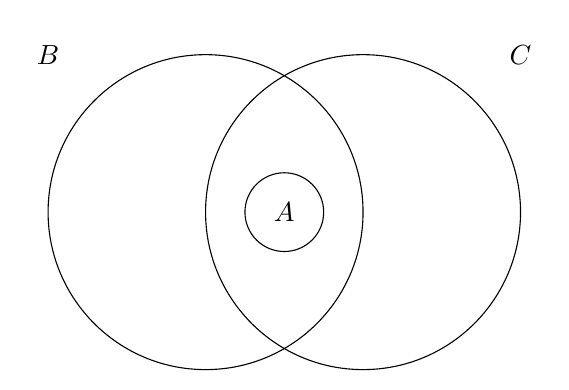
\begin{tikzpicture}[scale=1]
  \draw (-1,0) circle (2);
  \draw ( 1,0) circle (2);

  \node at (-3,2) {$B$};
  \node at ( 3,2) {$C$};

  \draw (0,0) circle (0.5);
  \node at (0,0) {$A$};
\end{tikzpicture}

\end{solution}

\begin{problem}{\S 2.1: 20}
What is the cardinality of each of the following sets?
\begin{enumerate}
    \item[(a)] $\emptyset$
    \item[(b)] $\{ \emptyset \}$
    \item[(c)] $\{ \emptyset, \{ \emptyset \} \}$
    \item[(d)] $\{ \emptyset, \{ \emptyset \}, \{ \emptyset, \{ \emptyset \} \} \}$
\end{enumerate}
\end{problem}

\begin{solution}
Following are the cardinality of each set
\begin{enumerate}
    \item[(a)] zero
    \item[(b)] one
    \item[(c)] two
    \item[(d)] three
\end{enumerate}
\end{solution}

\begin{problem}{\S 2.1: 26}
Show that if $A \subseteq C$ and $B \subseteq D$, then $A \times B \subseteq C \times D.$
\end{problem}

\begin{proof}
Let $a \in A$ and $b \in B$. By definition of cartesian product, $A \times B = \{(a,b)\}$. It is given that $A \subseteq C$ and $B \subseteq D$, then $a \in C$ and $b \in D$. So $\forall a,b, (a,b) \in C \times D$. Hence $A \times B \subseteq D \times D$
\end{proof}

\begin{problem}{\S 2.1: 32(a,c)}
Let $A = \{ a, b, c \}$, $B = \{ x, y \}$, and $C = \{ 0, 1 \}$. Find the following Cartesian products.
\begin{enumerate}
    \item[(a)] $A \times B \times C$ \item[(c)] $C \times A \times B$
\end{enumerate}
\end{problem}

\begin{solution}
$$
\begin{aligned}
A \times B \times C 
= \{& (a,x,0),(a,x,1),(a,y,0),(a,y,1),\\
    & (b,x,0),(b,x,1),(b,y,0),(b,y,1),\\
    & (c,x,0),(c,x,1),(c,y,0),(c,y,1)\} 
\end{aligned}
$$

$$
\begin{aligned}
C \times A \times B
= \{& (0,a,x),(0,a,y),(0,b,x),(0,b,y),\\
    &(0,c,x),(0,c,y),(1,a,x),(1,a,y), \\ 
    &(1,b,x),(1,b,y),(1,c,x),(1,c,y)\}
\end{aligned}
$$

\end{solution}

\begin{problem}{\S 2.2: 4}
Let $A = \{ a, b, c, d, e \}$ and $B = \{ a, b, c, d, e, f, g, h \}$. Find:
\begin{enumerate}
    \item[(a)] $A \cup B$.
    \item[(b)] $A \cap B$.
    \item[(c)] $A - B$.
    \item[(d)] $B - A$.
\end{enumerate}
\end{problem}

\begin{solution}
\mbox{}\par
    \begin{enumerate}
        \item[(a)] $A \cup B = \{ a,b,c,d,e,f,g,h \}$.
        \item[(b)] $A \cap B = \{a,b,c,d,e\}$.
        \item[(c)] $A - B = \emptyset$.
        \item[(d)] $B - A = \{f,g,h\}$.
\end{enumerate}
\end{solution}
\begin{problem}{\S 2.2: 14}
Find the sets $A$ and $B$ if $A - B = \{ 1, 5, 7, 8 \}$, $B-A = \{ 2, 10 \}$, and $A \cap B = \{ 3, 6, 9 \}$.
\end{problem}

\begin{solution}
\mbox{}\par

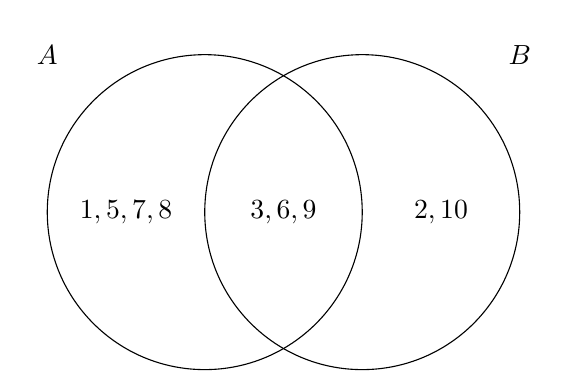
\begin{tikzpicture}[scale=1]
  \draw (-1,0) circle (2);
  \draw ( 1,0) circle (2);

  \node at (-3,2) {$A$};
  \node at ( 3,2) {$B$};

  \node at (-2,0) {$1,5,7,8$};
  \node at ( 2,0) {$2,10$};
  
  \node at (0,0) {$3,6,9$};
\end{tikzpicture}

As presented by the graph, $A = \{1,5,7,8,3,6,9\}, B = \{ 3,6,9,2,10\}$

\end{solution}

\begin{problem}{\S 2.2: 15}
Prove the second De Morgan law in Table 1 by showing that if $A$ and $B$ are sets, then $\overline{A \cup B} = \overline{A} \cap \overline{B}$ (a) showing each side is a subset of the other side and (b) by using a membership table.
\end{problem}

\begin{solution}
\begin{proof}
Method 1:  

For the first method we need to show that $\overline{A \cup B} \subseteq \overline{A} \cap \overline{B}$ and $ \overline{A} \cap \overline{B} \subseteq \overline{A \cup B}  $. 

Starting with $\overline{A \cup B} \subseteq \overline{A} \cap \overline{B}$:

Let $x \in \overline{A\cup B}$, then $x \notin A $ and $x \notin B$. Then $x \in \overline{A} \cap \overline{B}$, which means $\overline{A \cup B} \subseteq \overline{A} \cap \overline{B}$.

Then to prove $ \overline{A} \cap \overline{B} \subseteq \overline{A \cup B}  $ : 

Let $ x \in \overline{A} \cap \overline{B}$, then $ x \in \overline{A} $ and $ x \in \overline{B}$. Then $ x \notin A$ and $ x \notin B$. So $x \notin A \cup B$ which means $ x \in \overline{A \cup B}$. Hence $ \overline{A} \cap \overline{B} \subseteq \overline{A \cup B}  $.  

Because $\overline{A \cup B} \subseteq \overline{A} \cap \overline{B}$ and $ \overline{A} \cap \overline{B} \subseteq \overline{A \cup B}  $, $\overline{A \cup B} = \overline{A} \cap \overline{B}$ .

\end{proof}



\begin{proof}
Method 2: 

In this method, we list the membership table of both sets and if the columns of both sets are identical, both sets are equivalent.
 
\begin{tabular}{ccccccc}
$A$ & $B$ & $A \cup B$ & $\overline{A \cup B}$ & $\overline{A}$ & $\overline{B} $ & $\overline{A} \cap \overline{B}$ \\
\hline\\
1 & 1 & 1 & 0 & 0 & 0 & 0\\
1 & 0 & 1 & 0 & 0 & 1 & 0\\
0 & 1 & 1 & 0 & 1 & 0 & 0\\
0 & 0 & 0 & 1 & 1 & 1 & 1
\end{tabular}

From the table we can tell that $ \overline{A \cup B}$ and $ \overline{A} \cap \overline{B}$ are identical in columns. Hence $\overline{A \cup B} = \overline{A} \cap \overline{B}$. 
    
\end{proof}
\end{solution}

\begin{problem}{\S 2.2: 24}
Let $A, B,$ and $C$ be sets. Show that $(A-B)-C = (A-C)-(B-C)$.
\end{problem}

\begin{solution}
We are checking the membership table of both left side and right side of the equation we need proof. If colomns of $(A-B)-C$ is the same as $(A-C)-(B-C)$
\newline

\begin{tabular}{cccccccc}
$A$ & $B$ & $C$ & $A - B$ & $ (A-B)-C $ & $A-C$ & $B-C $ & $(A-C)-(B-C)$ \\
\hline\\
1 & 1 & 1 & 0 & 0 & 0 & 0 & 0\\
1 & 1 & 0 & 0 & 0 & 1 & 1 & 0\\
1 & 0 & 1 & 1 & 0 & 0 & 0 & 0\\
1 & 0 & 0 & 1 & 1 & 1 & 0 & 1\\
0 & 1 & 1 & 0 & 0 & 0 & 0 & 0\\
0 & 1 & 0 & 0 & 0 & 0 & 1 & 0\\
0 & 0 & 1 & 0 & 0 & 0 & 0 & 0\\
0 & 0 & 0 & 0 & 0 & 0 & 0 & 0

\end{tabular}

As the columns of both sides of equation are equivalent, $(A-B)-C = (A-C)-(B-C)$.
 
\end{solution}

\begin{problem}{\S 2.2: 26}
Draw the Venn diagrams for each of the following combinations of the sets $A,B,$ and $C$.
\begin{enumerate}
    \item[(a)] $A \cap (B \cup C)$
    \item[(b)] $\overline{A} \cap \overline{B} \cap \overline{C}$
    \item[(c)] $(A-B) \cup (A-C) \cup (B-C)$
\end{enumerate}
\end{problem}

\begin{solution}
\mbox{}\par

(a)

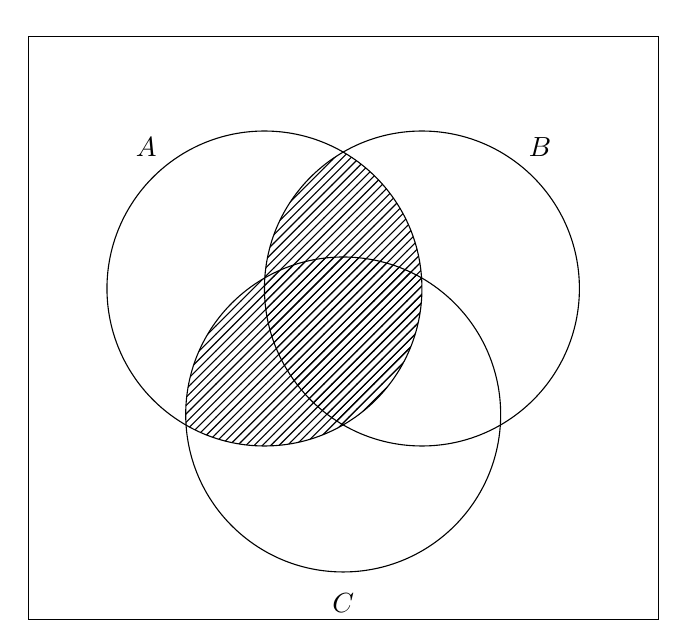
\begin{tikzpicture}

\begin{scope}
    \clip (-1,0) circle (2);   % restrain in A
    \fill[pattern=north east lines] ( 1,0) circle (2); % B
    \fill[pattern=north east lines] ( 0,-1.6) circle (2); % C
\end{scope}

    \draw ( -4, -4.2) rectangle (4,3.2);
    \draw (-1,0) circle (2); %A
    \draw ( 1,0) circle (2); %B
    \draw ( 0,-1.6) circle (2); %C
    
    \node at (-2.5,1.8) {$A$};
    \node at ( 2.5,1.8) {$B$};
    \node at ( 0,-4) {$C$};
    
\end{tikzpicture}

(b) 

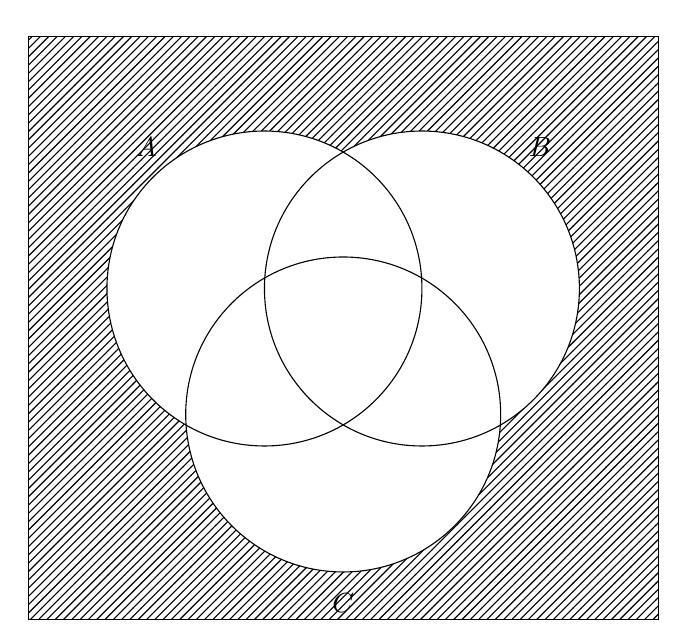
\begin{tikzpicture}

\begin{scope}[even odd rule]
    \fill[pattern=north east lines] 
        ( -4, -4.2) rectangle (4,3.2);
\end{scope}

\begin{scope}
    \fill[white] ( 1,0) circle (2); % A 
    \fill[white] ( -1,0) circle (2); % B 
    \fill[white] ( 0,-1.6) circle (2); % C
\end{scope}

    \draw ( -4, -4.2) rectangle (4,3.2);
    \draw (-1,0) circle (2); %A
    \draw ( 1,0) circle (2); %B
    \draw ( 0,-1.6) circle (2); %C
    
    \node at (-2.5,1.8) {$A$};
    \node at ( 2.5,1.8) {$B$};
    \node at ( 0,-4) {$C$};

\end{tikzpicture}

(c) 

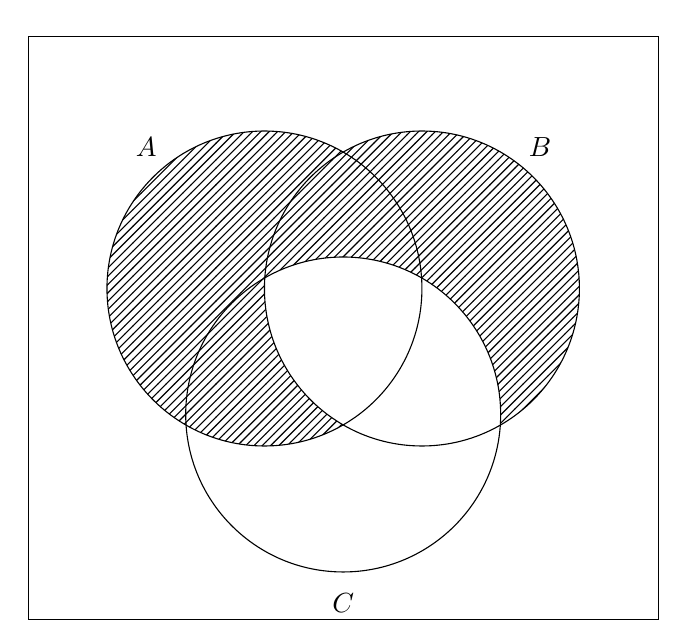
\begin{tikzpicture}

\begin{scope}
    \fill[pattern=north east lines] ( -1,0) circle (2); % fill A
\end{scope}

\begin{scope}
    \clip (-1,0) circle (2);   % restrain in A
    \fill[white] ( 1,0) circle (2); % B
\end{scope}

\begin{scope}
    \fill[pattern=north east lines] ( 1,0) circle (2); % fill B
\end{scope}

\begin{scope}
    \clip (1,0) circle (2);   % restrain in A
    \fill[white] ( 0,-1.6) circle (2); % C 
\end{scope}

    \draw ( -4, -4.2) rectangle (4,3.2);
    \draw (-1,0) circle (2); %A
    \draw ( 1,0) circle (2); %B
    \draw ( 0,-1.6) circle (2); %C
    
    \node at (-2.5,1.8) {$A$};
    \node at ( 2.5,1.8) {$B$};
    \node at ( 0,-4) {$C$};
    
\end{tikzpicture}

\end{solution}


\end{document}